% Centro y usuarios (docs/modelo-de-datos/centro-y-usuarios.md): el centro de acopio y sus usuarios.
\documentclass[tikz,border=0pt]{standalone}
% Estilo común de los diagramas de la documentación.
\usepackage[T1]{fontenc}
\usepackage[utf8]{inputenc}
\usepackage[sfdefault]{FiraSans}
\usepackage[scale=0.85]{FiraMono}
\usepackage{fontawesome5}
\usetikzlibrary{positioning,backgrounds,fit,arrows.meta,calc,matrix}

% Capa para los recuadros de zona: encima del fondo blanco y debajo de los equipos.
\pgfdeclarelayer{zonas}
\pgfsetlayers{background,zonas,main}

\definecolor{texto}{HTML}{262626}
\definecolor{azul}{HTML}{1F4E79}
\definecolor{naranja}{HTML}{C55A11}
\definecolor{gris}{HTML}{8C8C8C}

\tikzset{
  % Se aplica en cada tikzpicture: fondo blanco para que se lea en modo oscuro.
  diagrama/.style={
    font=\small, color=texto,
    background rectangle/.style={fill=white},
    show background rectangle, inner frame sep=14pt,
  },
  % Dispositivo con icono, título y descripción opcional.
  equipo/.style={
    draw=#1, fill=#1!10, line width=0.9pt, rounded corners=5pt,
    align=center, font=\footnotesize, inner sep=6pt, minimum width=3.1cm, minimum height=1.9cm,
  },
  equipo/.default=azul,
  % Recuadro que agrupa los equipos de un centro o una etapa.
  zona/.style={
    draw=#1, line width=0.8pt, rounded corners=8pt, inner sep=12pt,
  },
  zona/.default=gris,
  titulozona/.style={
    anchor=south west, font=\small\bfseries, text=#1, inner sep=3pt,
  },
  titulozona/.default=gris,
  enlace/.style={Latex-Latex, line width=0.9pt, draw=azul},
  copia/.style={-Latex, line width=1.1pt, draw=naranja},
  etiqueta/.style={font=\footnotesize, fill=white, inner sep=2pt, align=center},
  nota/.style={
    draw=#1, fill=#1!6, line width=0.7pt, rounded corners=4pt,
    font=\footnotesize, align=center, inner sep=5pt,
  },
  nota/.default=gris,
}

% \equipotexto{icono}{título}{descripción}
% La descripción usa el tamaño de letra del nodo, porque TikZ no conserva un cambio
% de tamaño después de \\ ni admite \\ dentro de un grupo.
\newcommand{\equipotexto}[3]{{\Large #1}\\[3pt]{\small\bfseries #2}\\[1pt]#3}

% Tabla del modelo de datos: una fila por campo (nombre, tipo y notas).
% Las celdas se nombran <tabla>-<fila>-<columna>, para poder unir campos con flechas.
\tikzset{
  tabla/.style={
    matrix of nodes, draw=#1, fill=#1!6, line width=0.9pt, rounded corners=5pt,
    inner sep=5pt, row sep=0pt, column sep=8pt,
    nodes={anchor=west, font=\footnotesize, inner sep=2.2pt, text height=1.6ex, text depth=0.4ex},
    column 1/.style={nodes={font=\footnotesize\ttfamily}},
    column 2/.style={nodes={text=gris!70!black}},
    row 1/.style={nodes={font=\small\bfseries, text=#1, text depth=0.8ex}},
  },
  tabla/.default=azul,
  relacion/.style={-Latex, line width=0.9pt, draw=texto!70},
}
% \lineatitulo{tabla}: línea bajo el título de una tabla.
\newcommand{\lineatitulo}[1]{\draw[line width=0.6pt] (#1-1-1.south west -| #1.west) -- (#1-1-1.south -| #1.east);}


\begin{document}
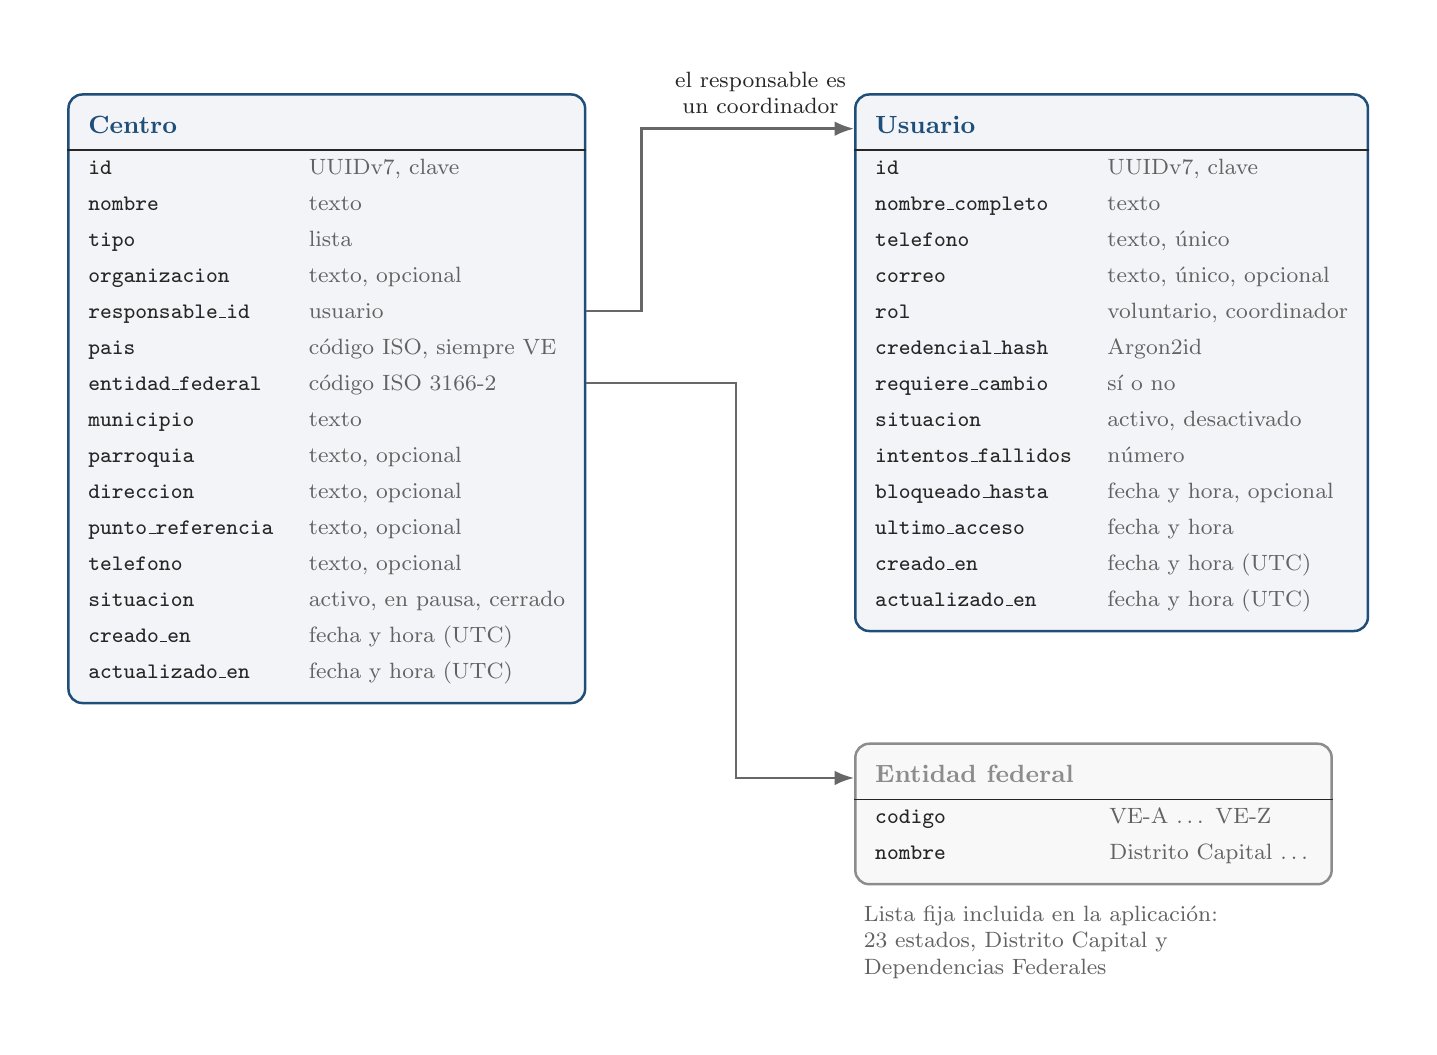
\begin{tikzpicture}[diagrama]

  \matrix (centro) [tabla] {
    Centro & \\
    id & UUIDv7, clave \\
    nombre & texto \\
    tipo & lista \\
    organizacion & texto, opcional \\
    responsable\_id & usuario \\
    pais & código ISO, siempre VE \\
    entidad\_federal & código ISO 3166-2 \\
    municipio & texto \\
    parroquia & texto, opcional \\
    direccion & texto, opcional \\
    punto\_referencia & texto, opcional \\
    telefono & texto, opcional \\
    situacion & activo, en pausa, cerrado \\
    creado\_en & fecha y hora (UTC) \\
    actualizado\_en & fecha y hora (UTC) \\
  };
  \lineatitulo{centro}

  \matrix (usuario) [tabla, right=3.4cm of centro.north east, anchor=north west] {
    Usuario & \\
    id & UUIDv7, clave \\
    nombre\_completo & texto \\
    telefono & texto, único \\
    correo & texto, único, opcional \\
    rol & voluntario, coordinador \\
    credencial\_hash & Argon2id \\
    requiere\_cambio & sí o no \\
    situacion & activo, desactivado \\
    intentos\_fallidos & número \\
    bloqueado\_hasta & fecha y hora, opcional \\
    ultimo\_acceso & fecha y hora \\
    creado\_en & fecha y hora (UTC) \\
    actualizado\_en & fecha y hora (UTC) \\
  };
  \lineatitulo{usuario}

  \matrix (entidad) [tabla=gris, below=1.4cm of usuario.south west, anchor=north west] {
    Entidad federal & \\
    codigo & VE-A \ldots\ VE-Z \\
    nombre & Distrito Capital \ldots \\
  };
  \lineatitulo{entidad}
  \node[font=\footnotesize, text=gris!70!black, anchor=north west, align=left]
    at ([yshift=-4pt]entidad.south west) {Lista fija incluida en la aplicación:\\23 estados, Distrito Capital y\\Dependencias Federales};

  \draw[relacion] (centro-6-2.east -| centro.east) -- ++(0.7,0) |- (usuario-1-1.west -| usuario.west)
    node[etiqueta, pos=0.78, above=3pt] {el responsable es\\un coordinador};
  \draw[relacion] (centro-8-2.east -| centro.east) -- ++(1.9,0) |- (entidad-1-1.west -| entidad.west);

\end{tikzpicture}
\end{document}
